\chapter{数据库设计}
\section{数据库环境说明}
本系统的数据库采用MySQL数据库系统

\section{数据库的命名规则}

名称的命名方式选用头字母大写(头分法)

不允许单词缩写,基本采用含义连拼的方式

表名是复数,大写

字段带上类型前缀(有利于数据库维护时对数据库进行操作与维护),中间用下划线分割:

EXP:

string——s

integer——i

long——l

char——c

double——lf

float——f

\section{逻辑设计}
\begin{figure}[H]
	\centering
	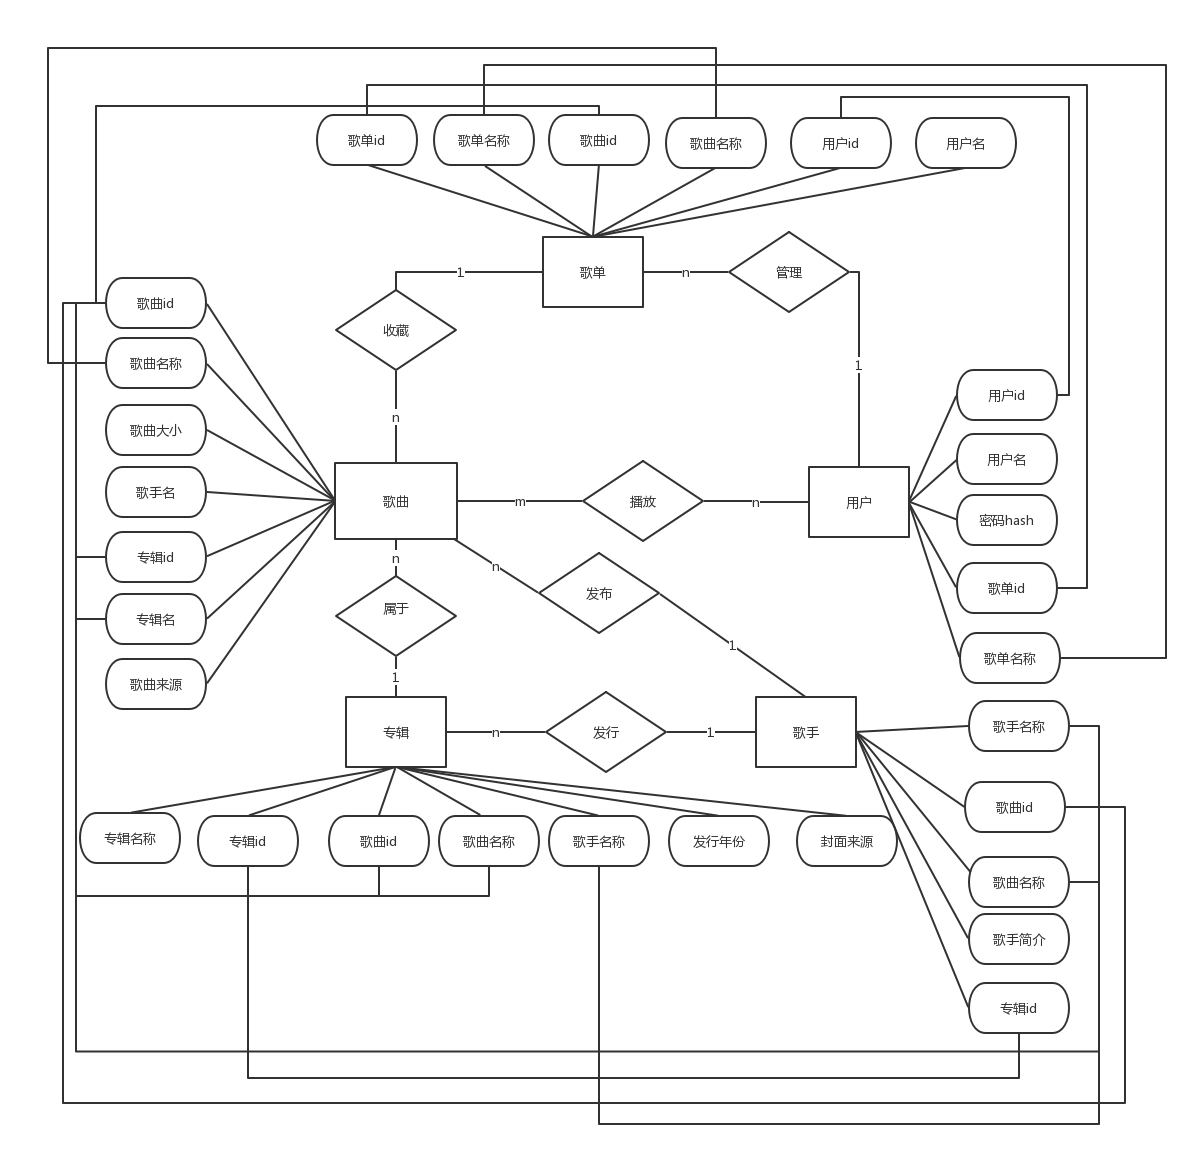
\includegraphics[width=10cm]{ER.png}
	\caption{逻辑设计图} 
	\label{fig:figure8er}
\end{figure}


\section{物理设计}
\subsection{数据库产品}
瑞典MySQL AB 公司的MySQL数据库,非分布式

\subsection{实体属性、类型、精度}



\subsubsection{歌曲数据表设计}
\begin{table}[htbp]
	\centering
	\caption{歌曲数据表Songs设计} \label{tab:songs-database}
	\begin{tabular}{|c|c|c|c|c|}
		\hline
		字段名 & 类型 & 大小 & 说明 & 备注 \\
		\hline
		s\_id & char & 64 & 歌曲的唯一标识符 & 主键\\
		\hline
		s\_name & char & 128 & 歌曲的名称 &  \\
		\hline
		f\_size & float & 1 & 歌曲文件的大小 & \\
		\hline
		s\_artist\_name & char & 64 & 歌手的名称 & 外键,来自Artists表 \\
		\hline
		s\_album\_id & char & 64 & 歌曲所属专辑的id & 外键,来自Albums表 \\
		\hline
		s\_album\_name & char & 128 & 歌曲所属专辑的名称 & \\
		\hline
		s\_source & char & 512 & 歌曲文件的来源,URL & \\
		\hline
	\end{tabular}
	\note{歌曲数据表Songs设计}
\end{table}

\subsubsection{专辑数据表设计}
\begin{table}[htbp]
	\centering
	\caption{专辑数据表Albums设计} \label{tab:albums-database}
	\begin{tabular}{|c|c|c|c|c|}
		\hline
		字段名 & 类型 & 大小 & 说明 & 备注 \\
		\hline
		s\_id & char & 64 & 专辑的唯一标识符 & 主键 \\
		\hline
		s\_song\_id & char & 64 & 专辑内某一歌曲的唯一标识符 & 外键,来自Songs表 \\
		\hline
		s\_song\_name & char & 128 & 专辑内某一歌曲的名称 & \\
		\hline
		s\_artist\_name & char & 64 & 专辑所属歌手的唯一标识符 & 外键,来自Artists表 \\
		\hline
		s\_publi\_date & date & 1 & 专辑发行日期 & \\
		\hline
		s\_cover\_src & char & 512 & 专辑封面的来源URL & \\
		\hline
	\end{tabular}
	\note{专辑数据表Albums设计}
\end{table}

\subsubsection{歌手数据表设计}
\begin{table}[htbp]
	\centering
	\caption{歌手数据表Artists设计} \label{tab:artists-database}
	\begin{tabular}{|c|c|c|c|c|}
		\hline
		字段名 & 类型 & 大小 & 说明 & 备注 \\
		\hline
		s\_name & char & 64 & 歌手的唯一标识符,也是歌手的名字 & 主键 \\
		\hline
		s\_song\_id & char & 64 & 歌手所发布歌曲的id & 外键,来自Songs表 \\
		\hline
		s\_song\_name & char & 128 & 歌手所发布歌曲的名称 & \\
		\hline
		s\_intro & char & 1024 & 歌手的简介信息 & \\
		\hline
	\end{tabular}
	\note{歌手数据表Artists设计}
\end{table}

\subsubsection{歌单数据表设计}
\begin{table}[htbp]
	\centering
	\caption{歌单数据表Lists设计} \label{tab:lists-database}
	\begin{tabular}{|c|c|c|c|c|}
		\hline
		字段名 & 类型 & 大小 & 说明 & 备注 \\
		\hline
		s\_id & char & 64 & 歌单的唯一标识符 & 主键 \\
		\hline
		s\_name & char & 128 & 歌单的名称 & \\
		\hline
		s\_song\_id & char & 64 & 歌单内某首歌曲的id & 外键,来自Songs表 \\
		\hline
		s\_song\_name & char & 128 & 歌单内某首歌曲的名称 & \\
		\hline
		s\_user\_id & char & 64 & 歌单所属用户的id & 外键,来自Users表\\
		\hline
		s\_user\_name & char & 128 & 歌单所属用户的用户名 & \\
		\hline
	\end{tabular}
	\note{歌单数据表Lists设计}
\end{table}

\subsubsection{用户数据表设计}
\begin{table}[htbp]
	\centering
	\caption{用户数据表Users设计} \label{tab:users-database}
	\begin{tabular}{|c|c|c|c|c|}
		\hline
		字段名 & 类型 & 大小 & 说明 & 备注 \\
		\hline
		s\_id & char & 64 & 用户的唯一标识符 & 主键 \\
		\hline
		s\_name & char & 128 & 用户名 & \\
		\hline
		s\_passwd & char & 512 & 用户密码的hash值 & \\
		\hline
		s\_list\_id & char & 64 & 用户的歌单的id & 外键,来自Lists表 \\
		\hline
		s\_list\_name & char & 128 & 用户歌单的名称 & \\
		\hline
	\end{tabular}
	\note{用户数据表Users设计}
\end{table}

\section{安全性设计}
备份和容灾设计。

设置一份与生产环境一致的容灾节点,利用磁盘介质在容灾节点保留一份生产系统每天的原始数据

在应用层面上,本地节点使用Cluster Server实现主机高可用性,防止主机故障.

在数据层面山,在本地先形成一套主机系统和业务数据的磁盘备份,并每隔8小时在后台将本地备份数据复制到远程容灾节点(周期复制),异地节点恢复主节点数据,以实现主备节点的数据同步。 

主节点和灾备节点在硬盘上至少保持6个月内的系统历史数据。 

\section{数据库管理与维护说明}
对于数据库的维护,随时对数据库中的信息加以调试和保存备份。同样需要个工作人员进行系统的分析和用户的反馈,对系统进行升级以及功能的完善。同时保证系统安全有序的运行。